% TODO
% Sjekk bregni ch5 anngående relativ frekvensfeil. Bruk begreper.
% Trigger uncertainty i manualen. Regn "slew-rate" og les i manualen. 
% 1 delt på kvadratroten av antall samples som jeg har tatt gjennomsnitt over. Se skriv om allan 2 anggående hvitfasesteøy pga triggerkrets. 


\documentclass[11pt,english,a4paper]{article}

\usepackage[utf8]{inputenc}          % Allows UTF-8 encoded characters in the .tex-file.
\usepackage{babel,csquotes,textcomp} % Set LaTeX to structure the content following international academic standards.
\usepackage[titletoc,toc]{appendix}
\usepackage{subfig}

\usepackage{hyperref}
\usepackage{graphicx}
\usepackage{pdfpages}
\usepackage{listings}
\usepackage{wrapfig}
\usepackage{color,colortbl}
\usepackage{lettrine}
\usepackage[font={small,it}]{caption}
\usepackage{multirow}
\usepackage{tabularx}
\usepackage{footnote}
\usepackage{enumitem}
\usepackage{amsmath}

\usepackage{setspace}
\onehalfspacing

\usepackage[
    backend=biber,
    style=numeric
]{biblatex}
\addbibresource{refs.bib}

\lstset{ %
  basicstyle=\ttfamily\small,     
  backgroundcolor=\color{white},   % choose the background color
  breaklines=true,                 % automatic line breaking only at whitespace
  captionpos=b,                    % sets the caption-position to bottom
  commentstyle=\color{mygreen},    % comment style
  escapeinside={\%*}{*)},          % if you want to add LaTeX within your code
  keywordstyle=\color{blue},       % keyword style
  stringstyle=\color{mymauve},     % string literal style
}

\title{Lab report \\ Frequency Counters}
\author{Aril Schultzen}

\begin{document}
\maketitle
\tableofcontents
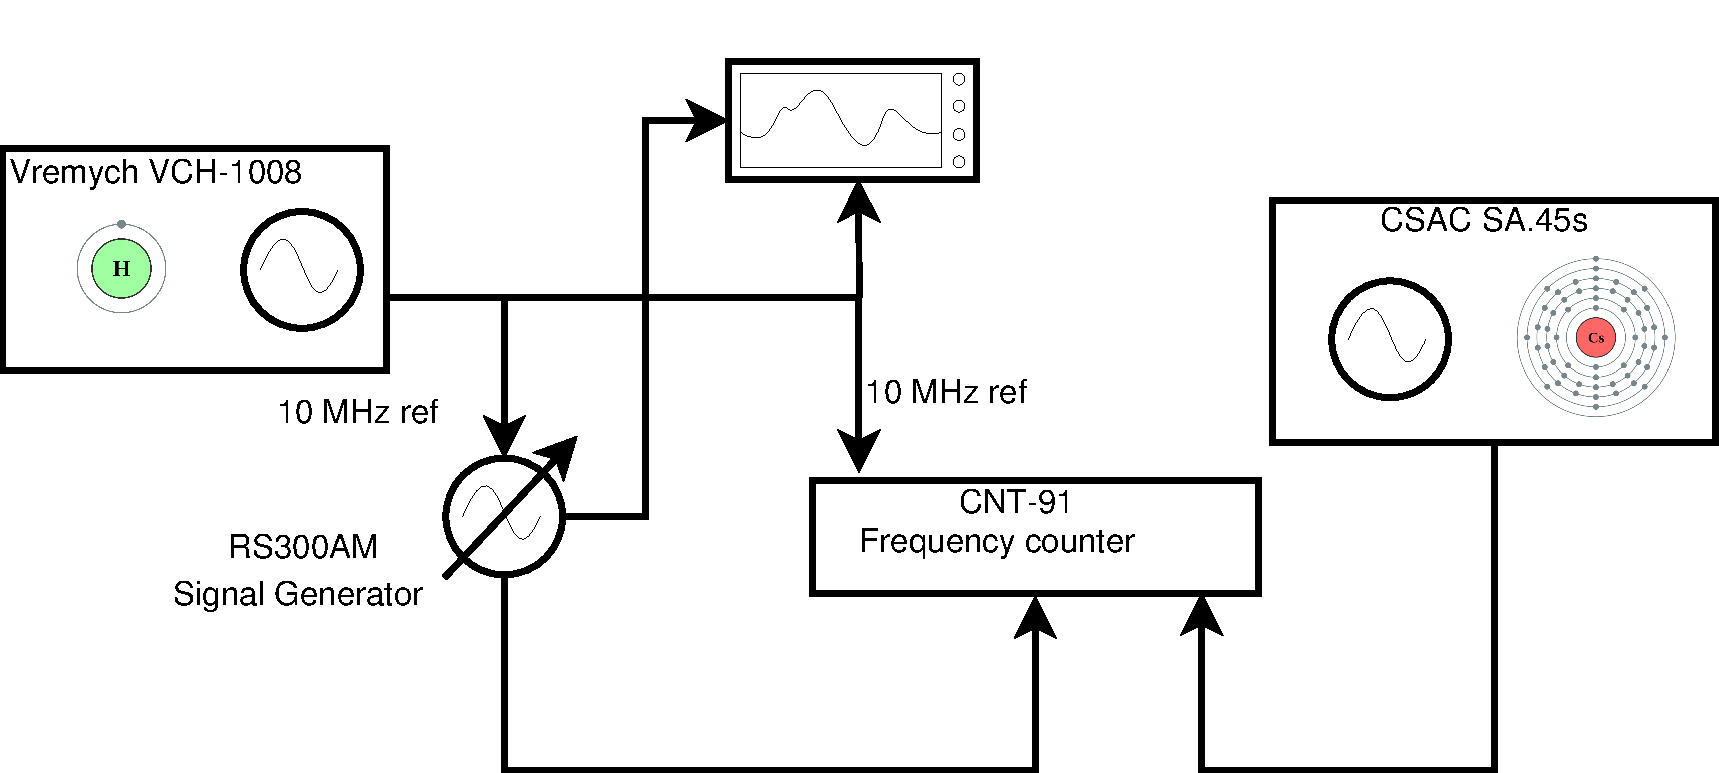
\includegraphics[width=1 \textwidth]{lab_report_diagram.pdf}


\section{Equipment}
\begin{itemize}
  \item Pendulum CNT-91, Frequency counter
  \item Rohde \& Scwarz 300AM, signal generator
  \item Tektronix MD0-4000-6 Oscilloscope
  \item Stopwatch, generic
  \item CSAC, oscillator to measure
  \item Passive Hydrogen maser, frequency reference
  \item RG-58 or RG223 cables
\end{itemize}

\section{Part A, frequency characterization}
\begin{figure}[!htb]
  \centering
  \subfloat[Oscilloscope capture 14:10:41]{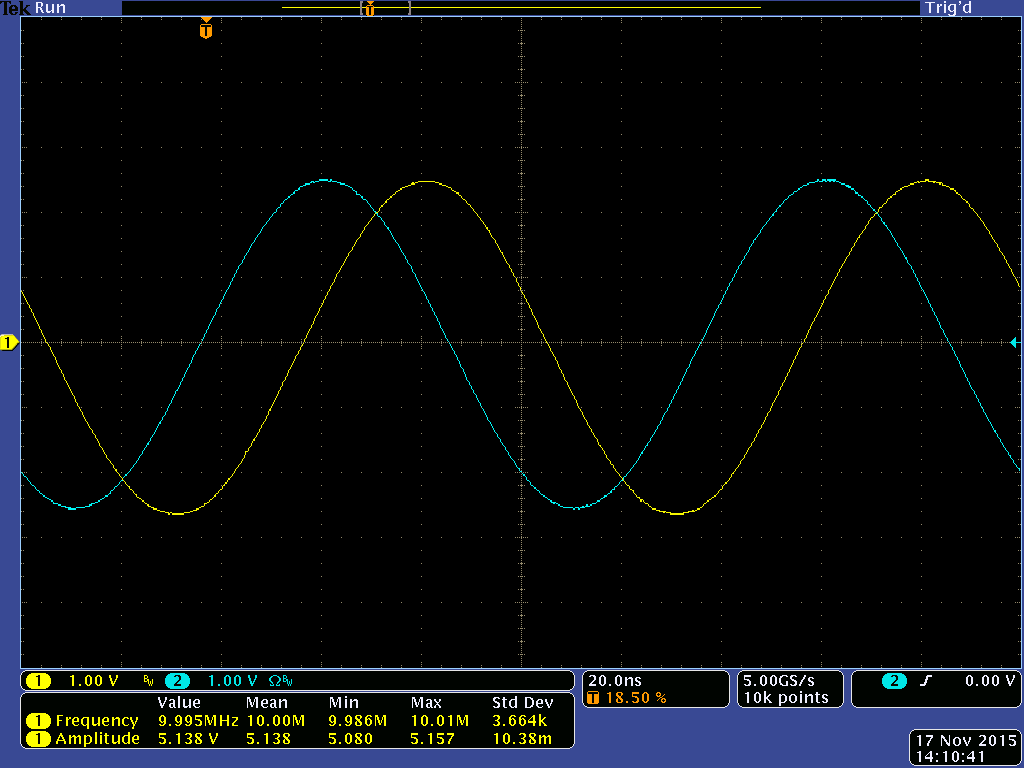
\includegraphics[width=0.5\textwidth]{tek00000.png}\label{fig:f1}}
  \hfill
  \subfloat[Oscilloscope capture 14:10:48]{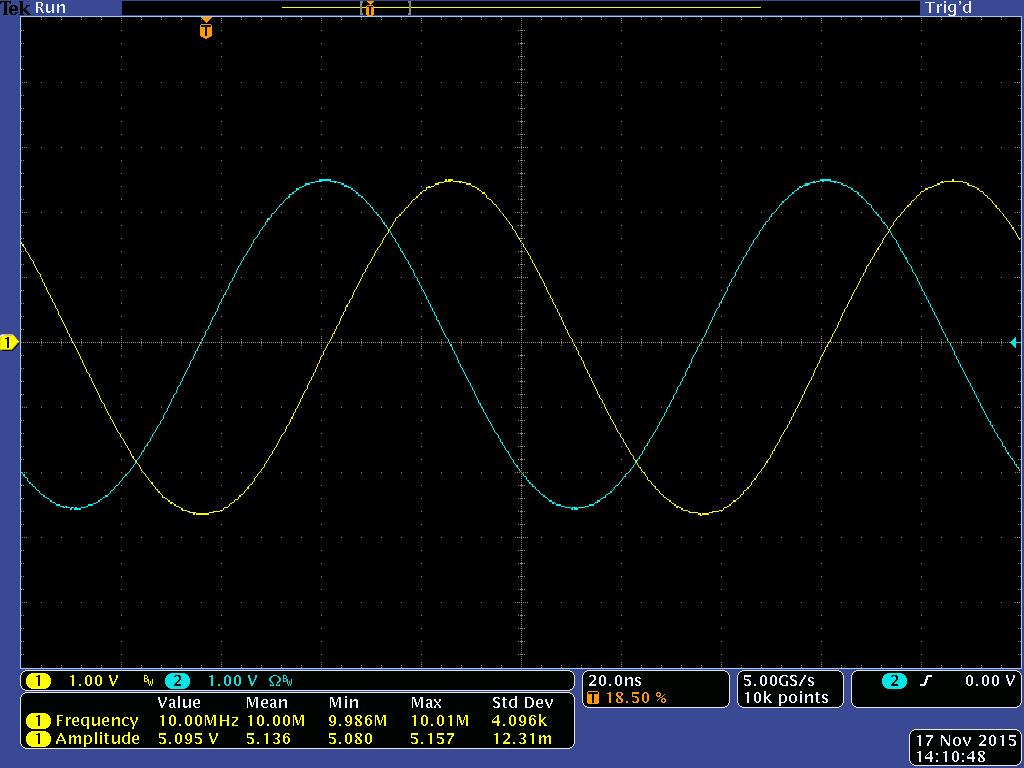
\includegraphics[width=0.5\textwidth]{tek00001.png}\label{fig:f2}}
  \caption{Oscilloscope captures}
\end{figure}
Figure \ref{fig:f1} and \ref{fig:f2} is two screenshots taken from the oscilloscope. The yellow line is the Passive hydrogen maser, the blue is the from the signal generator. The oscilloscope is triggering on the input from the signal generator. 

\subsection{Observations}
The two images (\ref{fig:f1} and \ref{fig:f2}) shows the yellow line moving towards the right. The reason the yellow line is moving to the right, is because the frequency of the signal from the generator is higher and therefor "arrives earlier" than the signal from the maser. When set to trigger on the maser instead, the effect is reversed, the blue line moves towards the left. The generator is in other words, a little fast. How fast you say? Each dotted square on the plot equals 20 ns. The squares are then divided into 5 parts at 4 ns each. During the 7 seconds that separate the two screenshots, the signal from the signal generator advanced by roughly 5.6 ns (or $\frac{5.6ns}{7s}=0.8ns/s$).

\subsection{Measuring relative frequency error}
The period for each of the signals are 100 ns. By measuring the time it took for the two signals to go from being in phase once to twice (in phase, out of phase, in phase again), a relative frequency error can be calculated:

\begin{displaymath}
\frac{period}{phase-in-out-in} = \frac{100 ns}{160 s} = 0.625 ns/s
\end{displaymath}
\newline
It's worth noting that the phase-in-out-in time was measured using my wristwatch and that the accuracy of the measurement was anything but accurate. This is not a problem since the oscillators where measured with extremely high resolution.
The same principle applies to the oscilloscope concerning its lack of external frequency reference.   
\newpage

\section{Part 2: Frequency counting: Resolution and trigger noise: BTB}
The setup was reconfigured:
\begin{center}
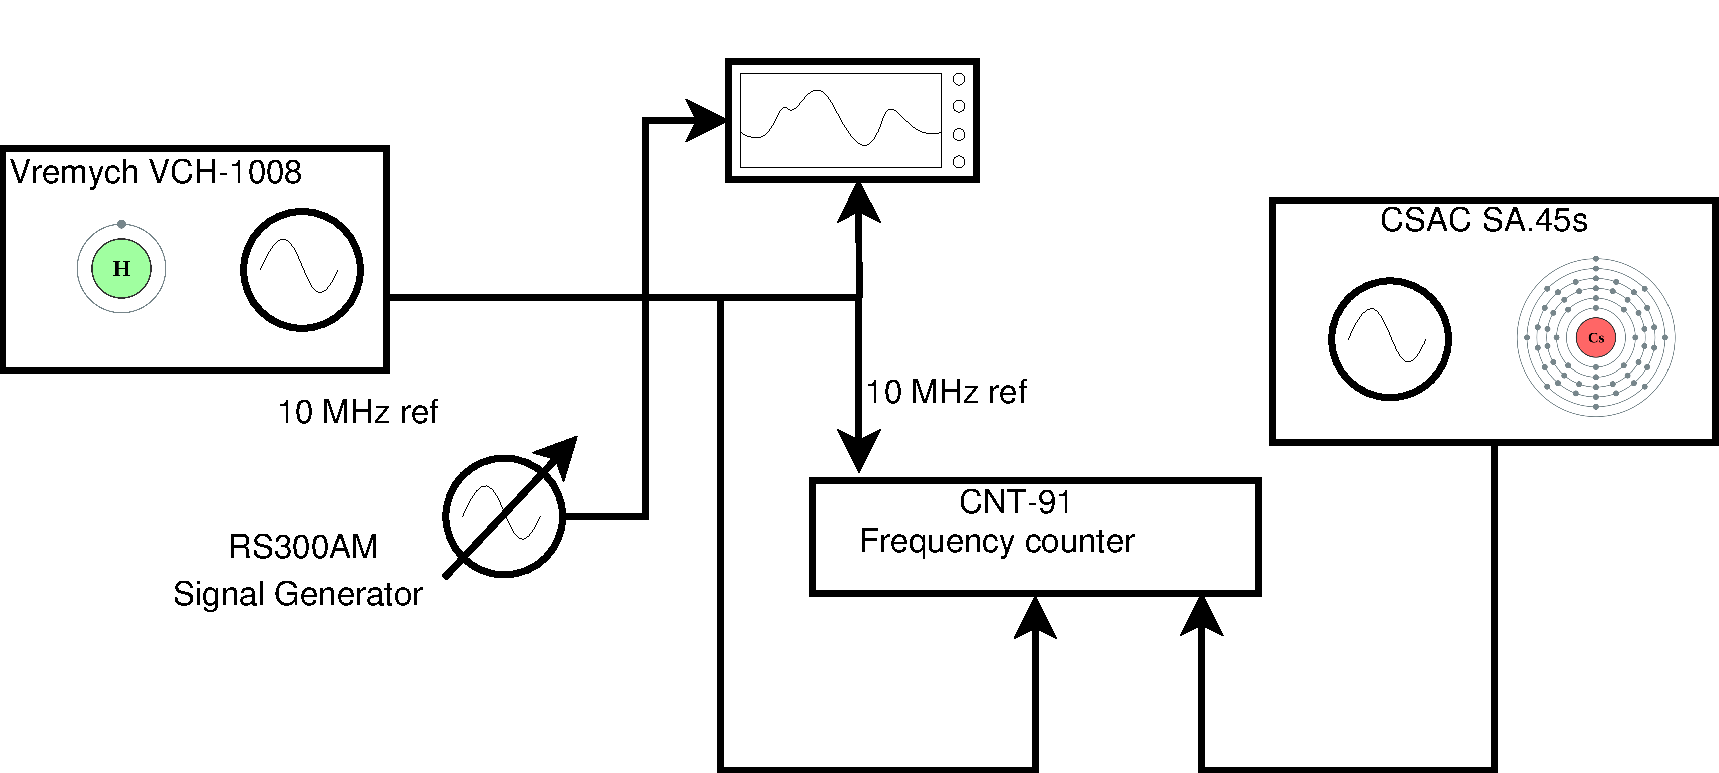
\includegraphics[width=1 \textwidth]{lab_report_diagram_del2.pdf}
\end{center}
The frequency counter now measures the maser (on input A) and uses it as reference. TimeView was then used to measure the frequency on input A, doing 200 samples with 1 s interval.

\subsection{Observations}
\subsubsection{Trigger resolution}
According to the User Manual for the CNT 9x Series, the resolution for Period A,B Back-to-Back is 50 ps rms. By observing the Allan deviation for the measurement (\ref{fig:allan_dev1}) the same can be observed: At the 1 second mark, the Allan Deviation is 8.23E-11 (around 82.3 ps) which seems about right considering:

\begin{displaymath}
 50 ps\sqrt{2}\approx 70.71 ps
\end{displaymath}

 Observing the slope, we are dealing with either white phase and or flicker noise (-1 slope). When studying the Modified Allan deviation for the same data (\ref{fig:mod_allan_dev1}), it becomes clear that the dominant type of noise is white noise (-3/2 slope).

\begin{figure}[]
  \centering
    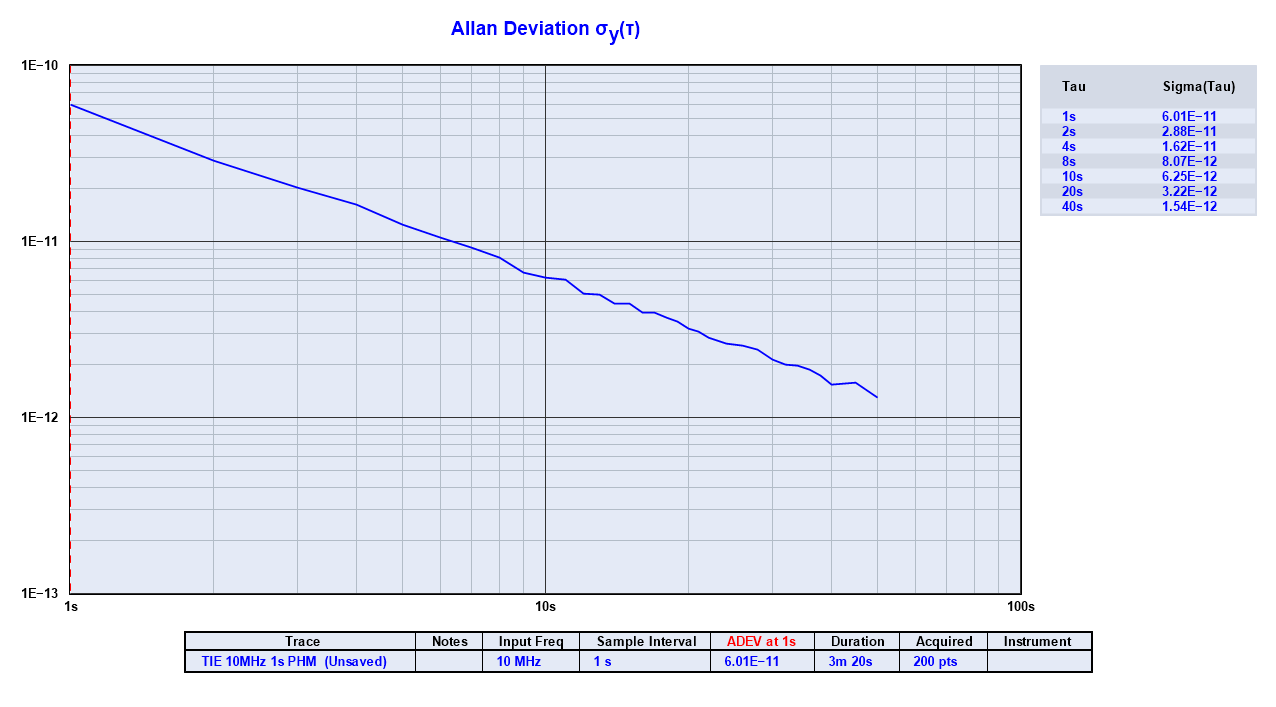
\includegraphics[width=1\textwidth]{phm10mhz1s_allan.png}
  \caption{Allan deviation for 200 samples at 1 s sample rate of 10MHz from the Passive Hydrogen maser.}
      \label{fig:allan_dev1}
\end{figure}

\begin{figure}[]
  \centering
    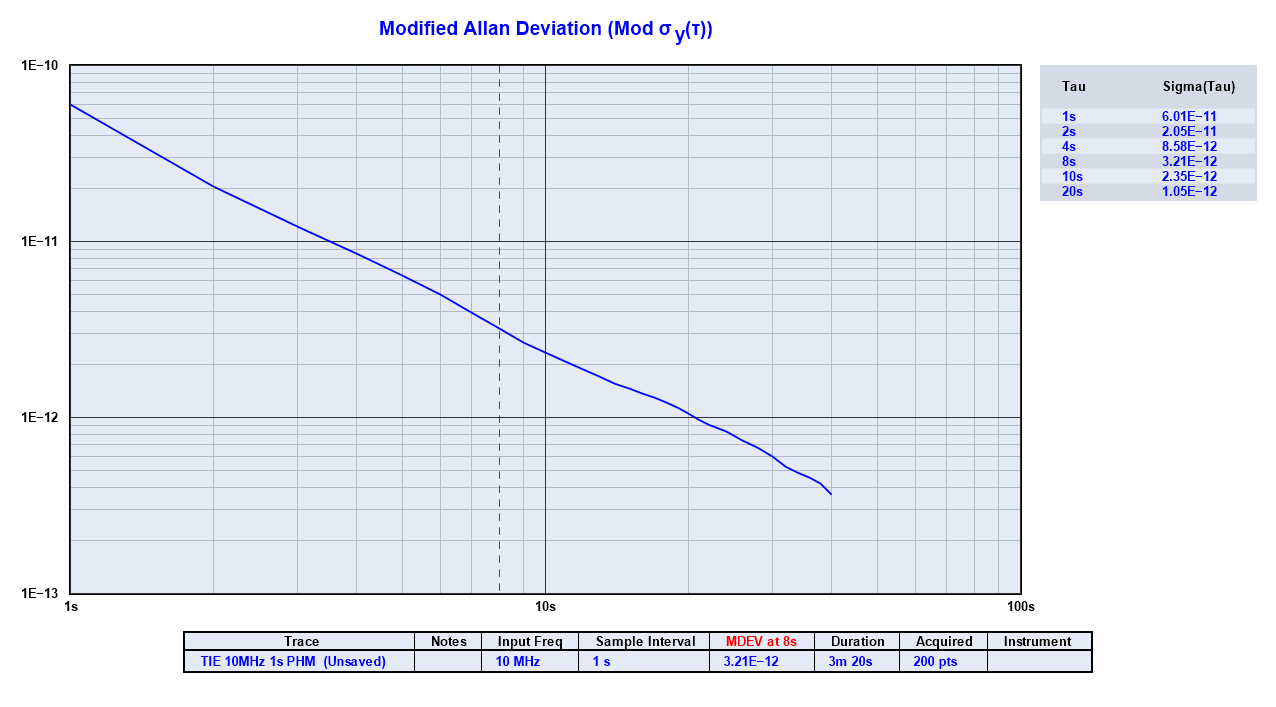
\includegraphics[width=1\textwidth]{phm10mhz1s_modified_allan.png}
  \caption{Modified Allan deviation for 200 samples at 1 s sample rate of 10MHz from the Passive Hydrogen maser.}
      \label{fig:mod_allan_dev1}
\end{figure}

\newpage
\subsubsection{Trigger level}
\begin{wrapfigure}{c}{0.45\textwidth}
  \centering
  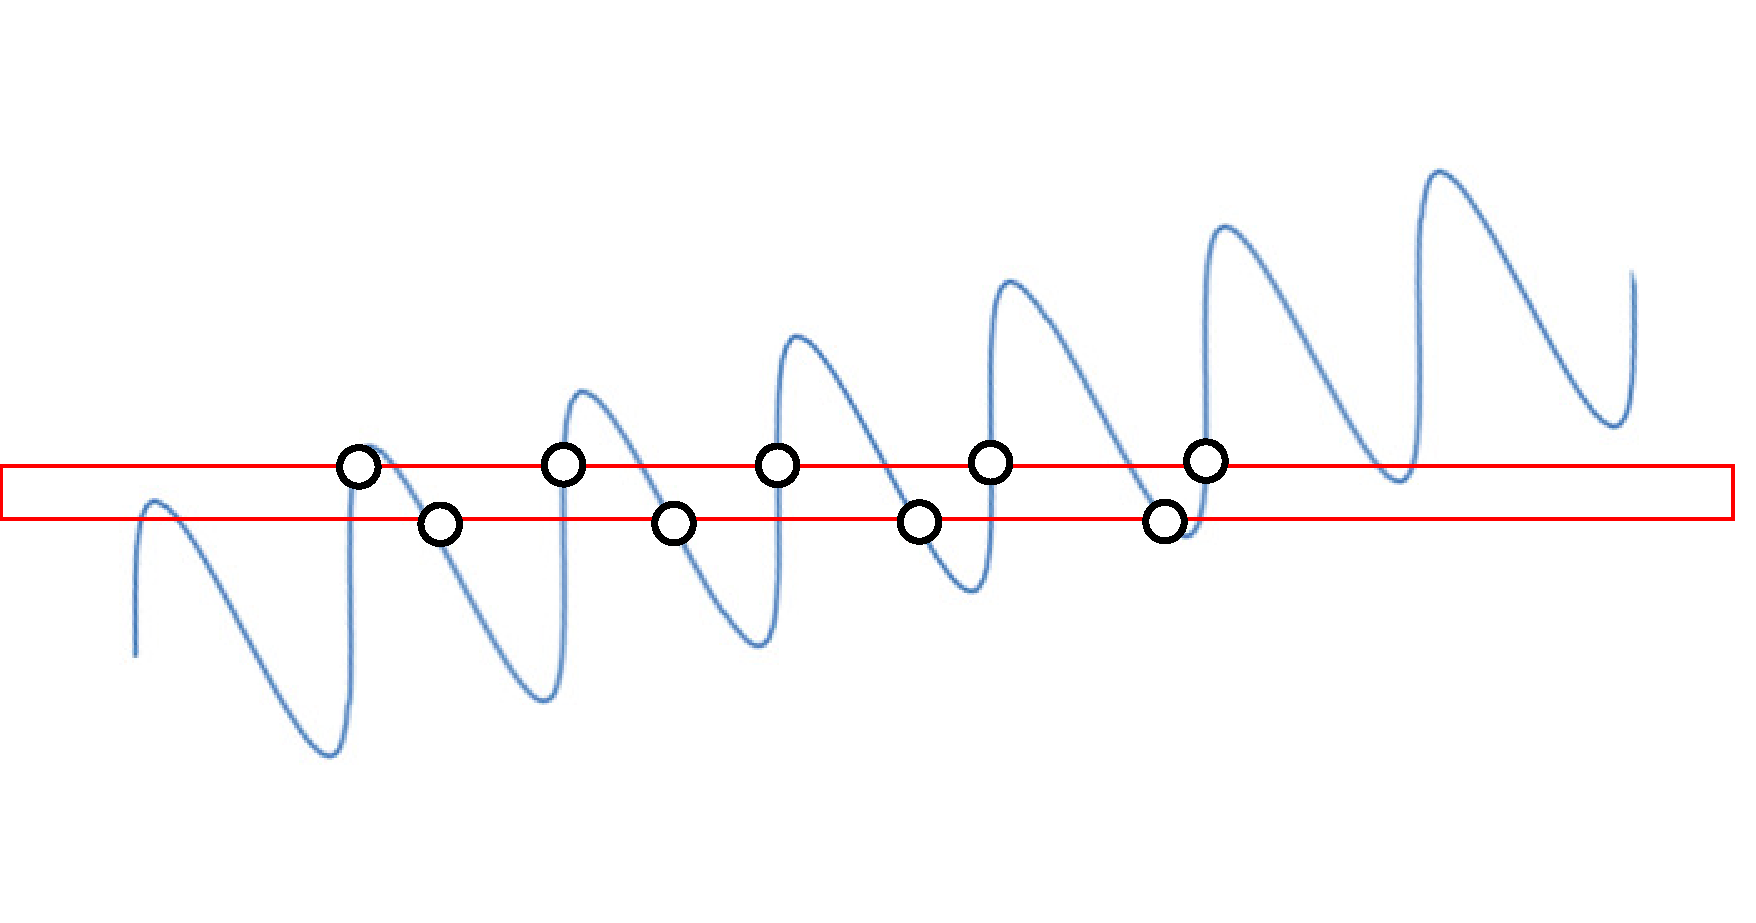
\includegraphics[width=0.40\textwidth]{hysteresis.pdf}
  \caption{Trigger counting multiple times as the noisy signal passes the hysteresis window}
    \label{fig:hysteresis}
\end{wrapfigure}
When raising the trigger level from 0 V to 1.2 V, more noise is introduced. This is because the slope of the signal is steeper at 0 V than at 1.2 V (closer to the middle of the sine wave) This means the signal is passing the hysteresis window at lower speed. The lower slope results in a less accurate trigging. In a really noisy signal, the signal can pass the hysteresis window more than once, thus generating erroneous counts (see figure \ref{fig:hysteresis}). This becomes evident when observing figure \ref{fig:PHM_10MHz_0V_1.2V_allan_dev} and \ref{fig:PHM_10MHz_0V_1.2V_freq_diff}. For the latter, figure \ref{fig:PHM_10MHz_0V_1.2V_freq_diff}, the spikes for the 1.2V plot shows the added uncertainty caused by the higher trigger level.

\begin{figure}[!htb]
  \centering
    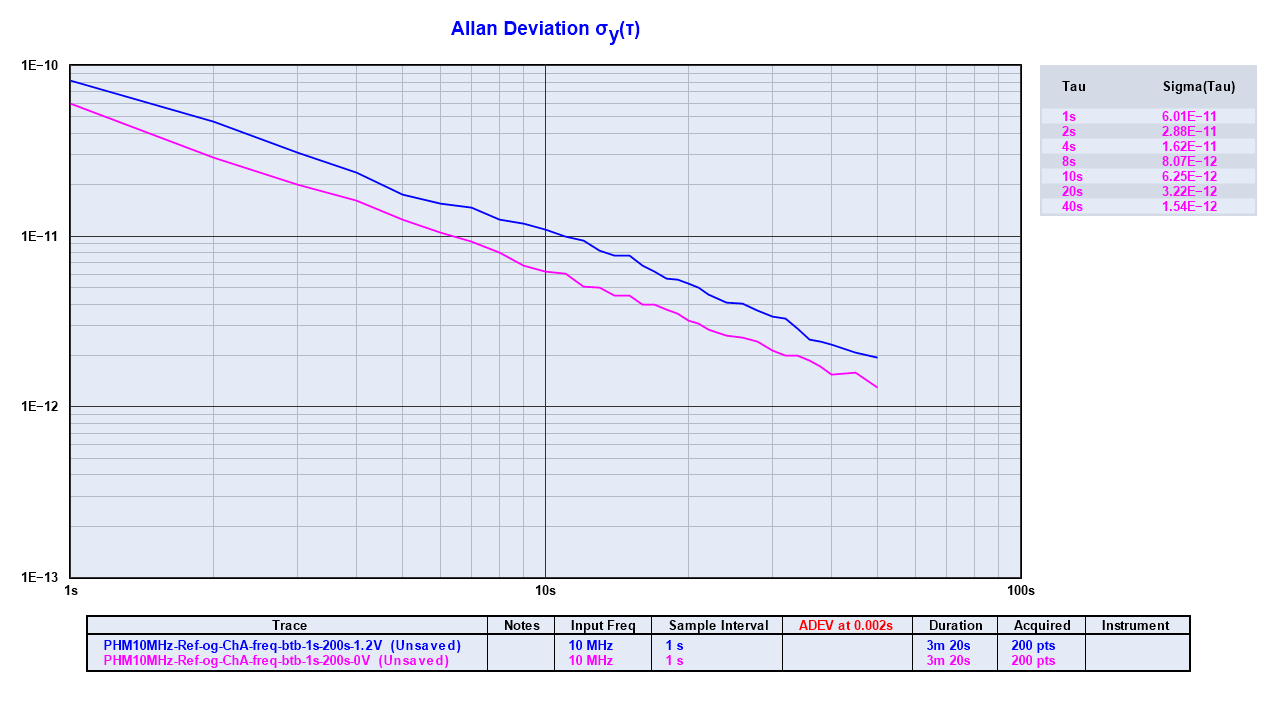
\includegraphics[width=1\textwidth]{PHM10MHz-Ref-og-ChA-freq-btb-1s-200s-allan.png}
    \caption{FBTB PHM 10 MHz at 1 s sample rate 200s total Allan Deviation. Blue plot is for 1.2V and pink is 0V}
        \label{fig:PHM_10MHz_0V_1.2V_allan_dev}
\end{figure}

\begin{figure}[!htb]
  \centering
    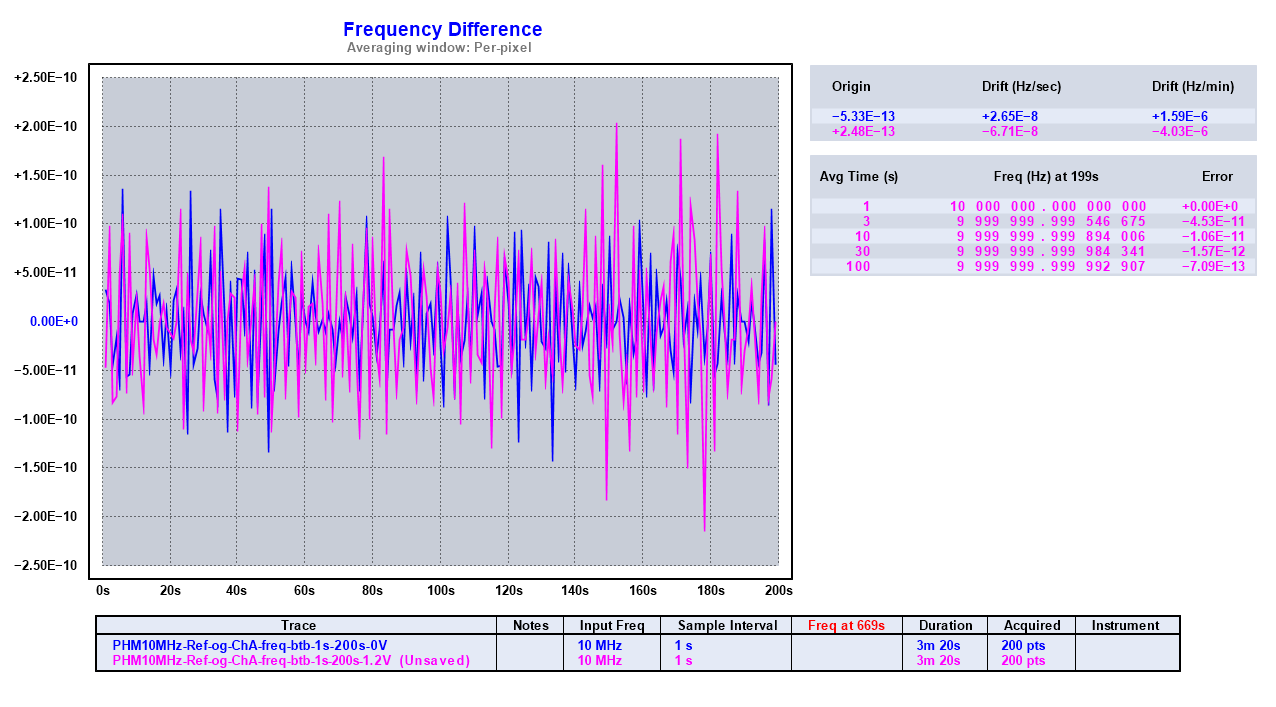
\includegraphics[width=1\textwidth]{PHM10MHz-Ref-og-ChA-freq-btb-1s-200s-frec_diff.png}
    \caption{FBTB PHM 10 MHz at 1 s sample rate 200s total Frequency Difference. Blue plot is for 1.2V and pink is 0V}
        \label{fig:PHM_10MHz_0V_1.2V_freq_diff}
\end{figure}

\newpage
\section{Part 2: Frequency counting: Resolution and trigger noise: TIE}
One of the advantages of the Modified Allan Deviation relative to regular Allan variance, is the ability to separate white phase noise from flicker noise. As we saw earlier, the dominating noise introduced by our frequency counter, was white noise. The white noise is a consequence of the limited resolution of the timers trigger. Since the triggers only allows a measurement to be accurate to within a certain resolution (in our case, $\approx$ 70.71 ps) everything beyond this point is anyones guess and results in uncorrelated noise. We used TimeView to make a Time Interval Error measurement of 200 000 samples at 1 ms sampling time. We also used a "smooth" function in TimeView that calculates a running average of 1000 samples. When comparing Allan Deviation for the smoothed measurement with the Modified Allan Deviation for the measurement without, the two meet around 1 s. At this point, the smoothing interval is at it's end. It also reveals some of the underlying mechanics of the Modified Allan Deviation which is actually realized by the use of averaging (hence the similarity).

\begin{figure}[!htb]
  \centering
  \subfloat[Cut out of screenshot showing the frequency difference for the measurement.]{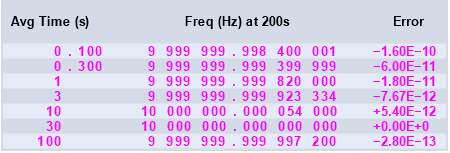
\includegraphics[width=0.5\textwidth]{tie_10mhz_phm_1ms_freq_diff_utklipp.png}\label{fig:freq_diff1}}
  \hfill
  \subfloat[Same cut out, but for the smoothed measurements. This measurement is clearly better.]{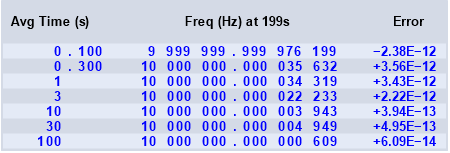
\includegraphics[width=0.5\textwidth]{tie_10mhz_phm_1ms_smooth_freq_diff_utklipp.png}\label{fig:freq_diff2}}
\end{figure}
As figure \ref{fig:freq_diff1} and \ref{fig:freq_diff2} shows, using an averaging technique when conducting measurements is obviously effective against white phase noise. At 1 s the Allan Deviation for the smoothed measurement was 1.56E-11 and the raw measurement was 6.24E-11. Though this might seem impressive, the technique can however be a little too aggressive when the signal is noise heavy and the variations are small. 

\begin{figure}[!htb]
  \centering
    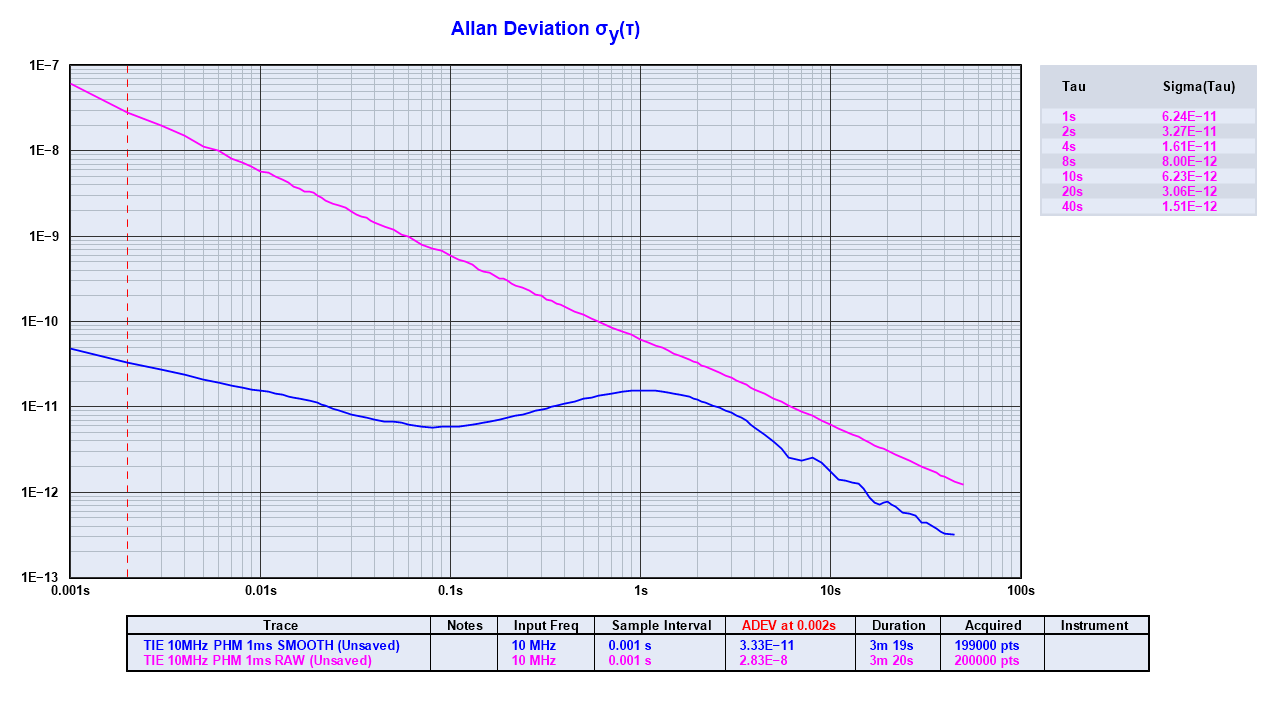
\includegraphics[width=1\textwidth]{tie_10mhz_phm_1ms_allan.png}
    \caption{TIE 10MHz PHM 1 ms sample rate Allan Deviation.}
        \label{fig:PHM_10MHz_allan_dev}
\end{figure}

\begin{figure}[!htb]
  \centering
    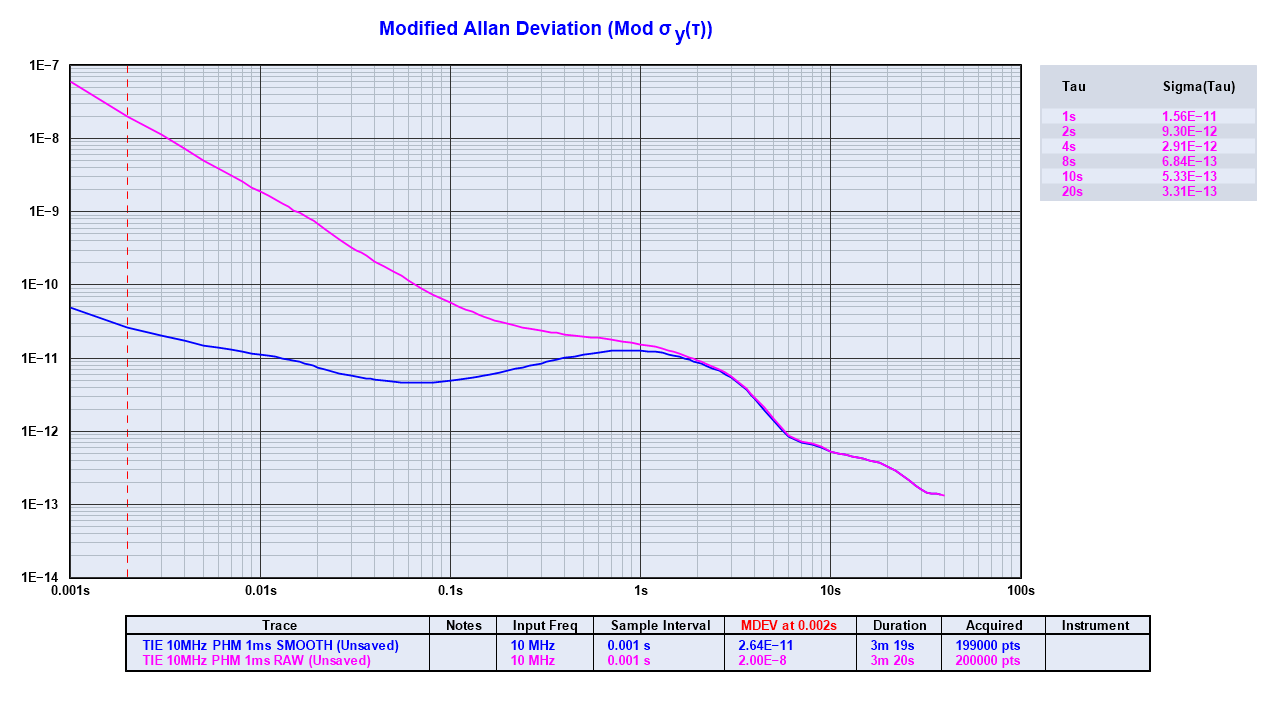
\includegraphics[width=1\textwidth]{tie_10mhz_phm_1ms_modified_allan.png}
    \caption{TIE 10MHz PHM 1 ms sample rate Modified Allan Deviation.}
        \label{fig:PHM_10MHz_mod_allan_dev}
\end{figure}

\begin{figure}[!htb]
  \centering
    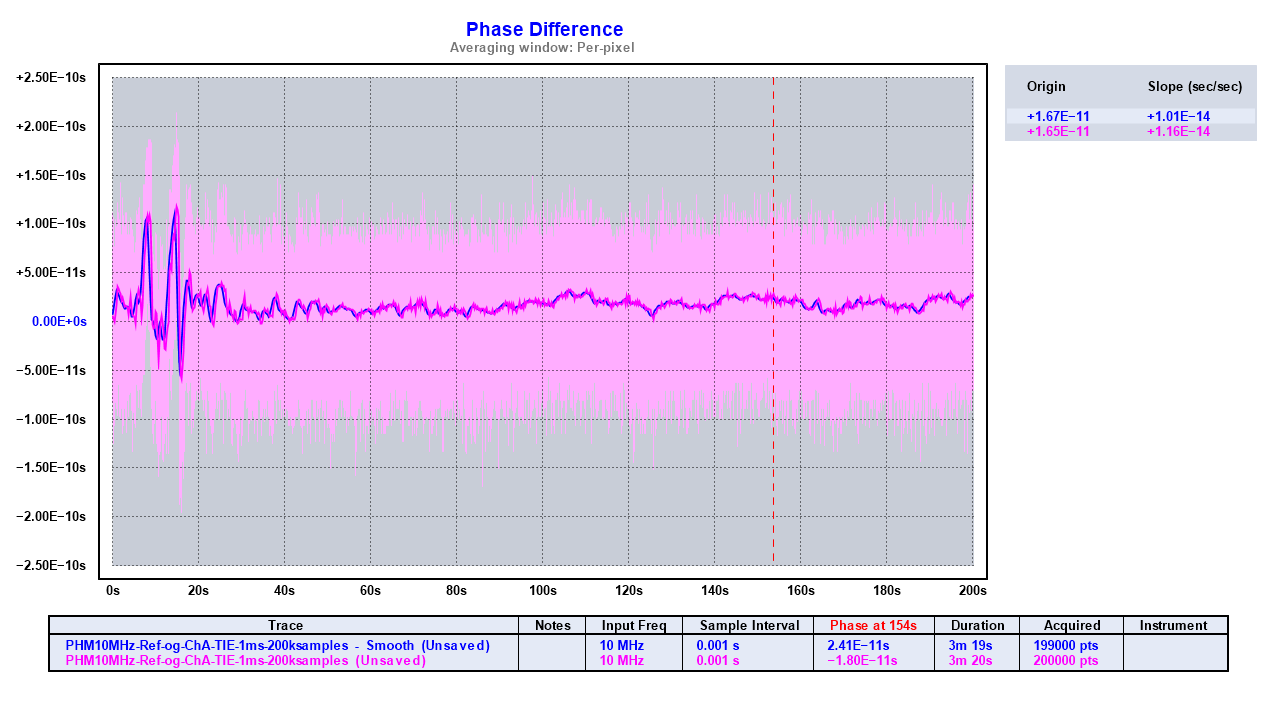
\includegraphics[width=1\textwidth]{part4_phase_diff.png}
    \caption{TIE 10MHz PHM 1 ms sample rate Phase Difference.}
        \label{fig:PHM_10MHz_phase_diff}
\end{figure}

\begin{figure}[!htb]
  \centering
    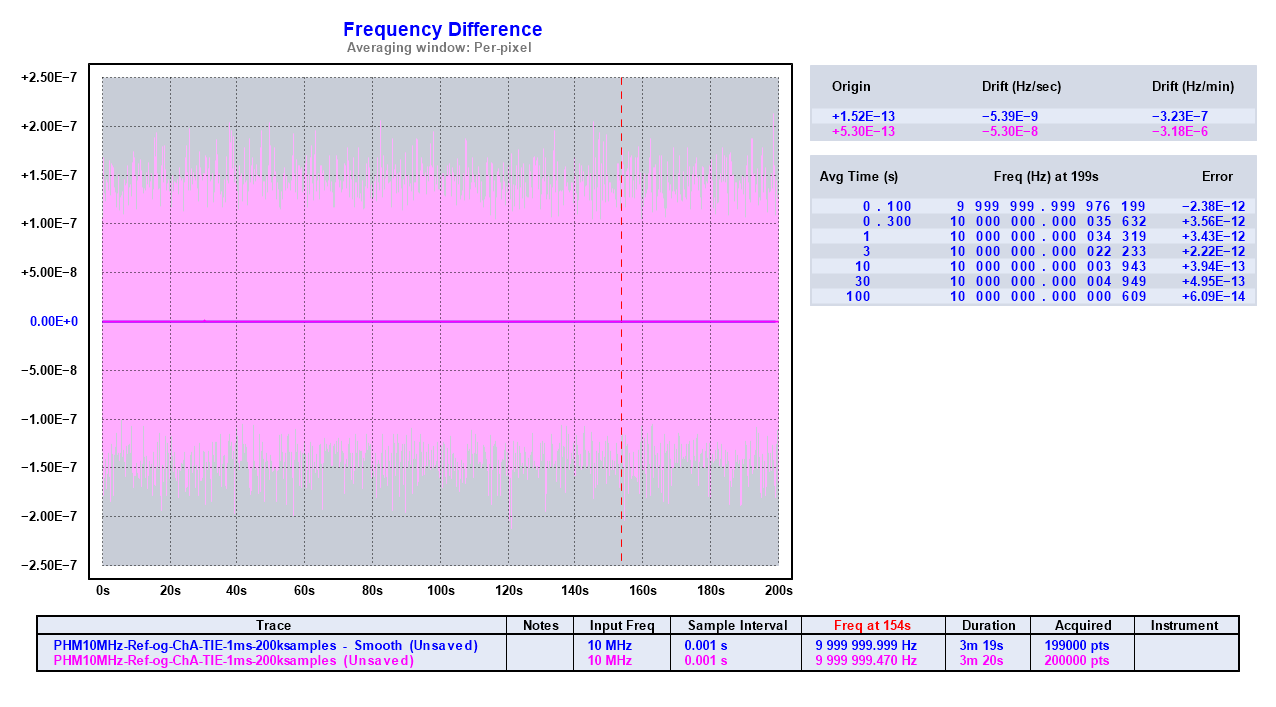
\includegraphics[width=1\textwidth]{part4_freq_diff.png}
    \caption{TIE 10MHz PHM 1 ms sample rate Frequency Difference.}
        \label{fig:PHM_10MHz_frequency_diff}
\end{figure}


\newpage
\section{Part 3: Frequency counting: Resolution and trigger noise: KHz and MHz}
The setup was reset to it's initial configuration. 
\begin{figure}[!htb]
  \centering
    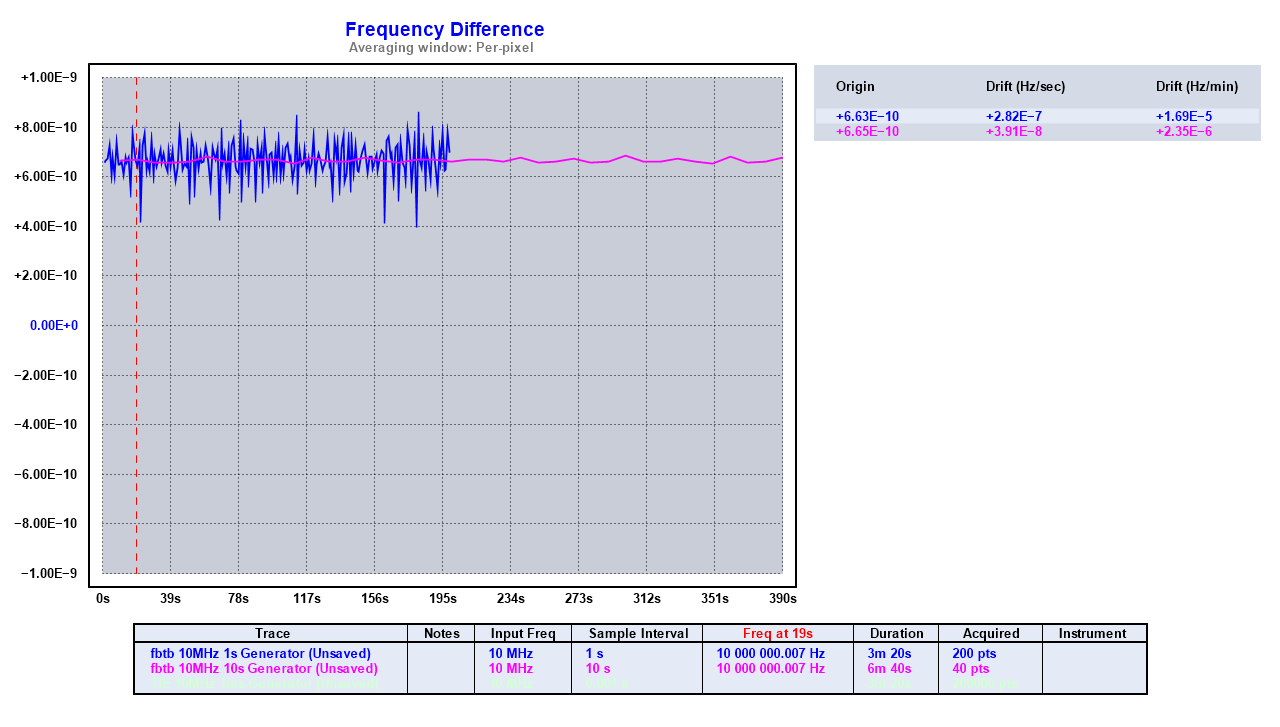
\includegraphics[width=1\textwidth]{freq_diff_del3.png}
   \caption{Screenshot showing the frequency difference of fbtb 10MHz and 10Khz from the signal generator}
  \label{fig:freq_diff_3}
\end{figure}
As figure \ref{fig:freq_diff_3} suggests, our earlier measurements using a wristwatch to determine the relative frequency error seems to be correct. These measurements though naive, is pretty accurate relative to the offset that the signal generator was configured to apply (+6.66E-10). By studying the Allan Deviation and the Modified Allan Deviation for the measurement, it becomes clear that using a sample rate of 10 seconds as opposed to 1 s, results in a more accurate measurement. The reason for this is that the trigger error divided by time is reduced when doing fewer measurements. Once again, the "Achilles Heel" of the setup seems to be the frequency counter. 

\begin{figure}[!htb]
  \centering
    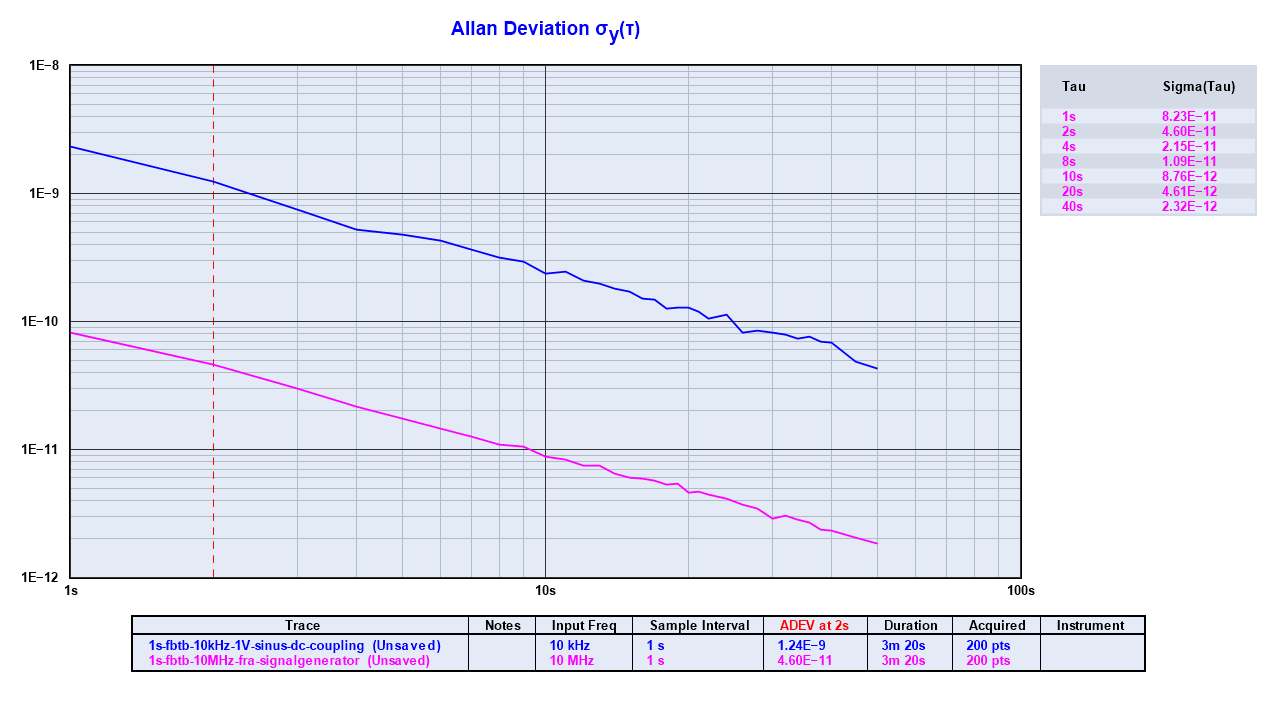
\includegraphics[width=1\textwidth]{fbtb_10mhzkhz_generator_allan.png}
    \caption{FBTB 10MHz/10KHz signal generator at 1s and 10 s sample rate Allan Deviation.}
        \label{fig:sg_10x_allan_dev}
\end{figure}

\begin{figure}[!htb]
  \centering
    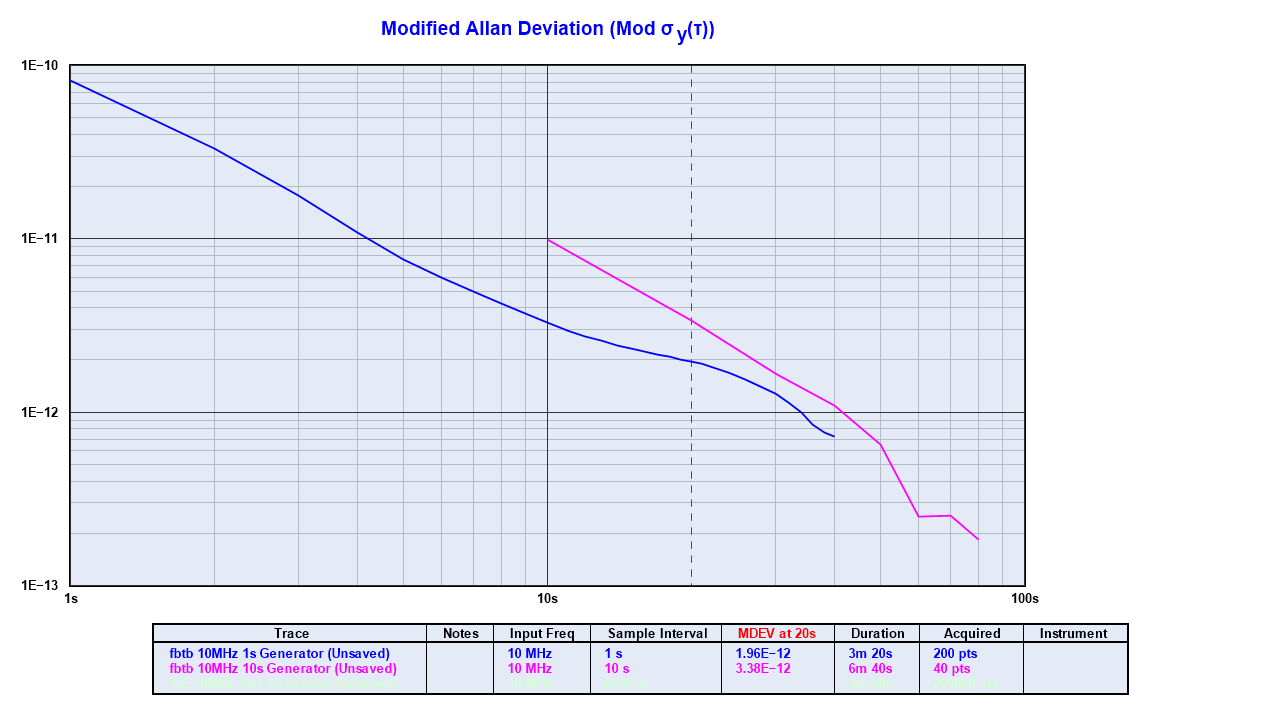
\includegraphics[width=1\textwidth]{fbtb_10mhzkhz_generator_mod_allan.png}\
  \caption{FBTB 10MHz/10Khz signal generator at 1s and 10 s sample rate Modified Allan Deviation.}
      \label{fig:sg_10x_mod_allan_dev}
\end{figure}

Figure \ref{fig:sg_10x_mod_allan_dev} is a screenshot of the Modified Allan Deviation for the following measurements:
\begin{itemize}
  \item TIE 10 KHz 1 ms sample rate 1V (blue)
  \item TIE 10 MHz 1 ms sample rate 5V (pink)
  \item TIE 10 KHz 1 ms sample rate 1V Smoothed (green)
\end{itemize}
As the figure suggests, the measurement taken at 10 MHz 5V (purple) is the most accurate. The CNT-9X manual specifies the random uncertainty (rms) under normal mode as:

\begin{displaymath}
U_{rnd}=\frac{\sqrt{E_{q}^2 + 2\cdot(Ess)^2}}{Measuring time}
\end{displaymath}
The Start Trigger Error (Ess) is defined as:
\begin{displaymath}
Ess = \sqrt{ E_{noise}^2 + E_{jitter}^2 }(s)
\end{displaymath}
The $E_{noise}$ is specified as:
\begin{displaymath}
E_{noise}\frac{\sqrt[]{V_{noise-input}^2 + V_{noise-signal}^2}}{inp.sign.slew rate(\frac{v}{s}) trig. point}(s)
\end{displaymath}
Now, because we are only interested in the counters characteristics, we can ignore $V_{noise-signal}$ and $E_{jitter}$. The manual also defines $E_{q} = 66$ ps rms and worst case $V_{noise-input} = 500 \mu V$ rms. The formula for calculating the slew rate is given as $2\pi Vf$, thus for the 10 KHz 1 V amplitude signal:
\begin{displaymath}
2\pi\cdot1 V\cdot10\cdot10^3 Hz = 62831.853 V/s
\end{displaymath}
And for the 10 MHz 5 V amplitude signal:
\begin{displaymath}
2\pi\cdot5 V\cdot10\cdot10^6 Hz = 314159265.358 V/s
\end{displaymath}
\newline
Calculating the random uncertainty for the 1V/10KHz signal:

\begingroup
\addtolength{\jot}{1em}
\begin{align}
E_{noise} = \frac{\sqrt{(500\cdot\sqrt{2})^2 + 0}}{62831.853V/s} = 0.011s\\
Ess = \sqrt{ (0.011)^2 + 0 } = 0.011s \\
Eq = 65\cdot10^{-12}\cdot\sqrt{2} = 9.122\cdot10^{-11}s \\
(Eq)^2 = 8.449\cdot10^{-21}s \\
U_{rnd} = \frac{\sqrt{8.449\cdot10^{-21} + 2\cdot(0.011)^2}}{200s} = 7.778\cdot10^{-5}s \\
\end{align}
\endgroup

For the 5V/10MHz (reusing some of the steps):

\begingroup
\addtolength{\jot}{1em}
\begin{align}
E_{noise} = \frac{\sqrt{(500\cdot\sqrt{2})^2} + 0}{314159265.358V/s} = 2.251\cdot10^{-6}s\\
U_{rnd} = \frac{\sqrt{8.449\cdot10^{-21} + 2\cdot(2.251\cdot10^{-6})^2}}{200s} = 1.592\cdot10^{-8}s
\end{align}
\endgroup


\begin{figure}[!htb]
  \centering
    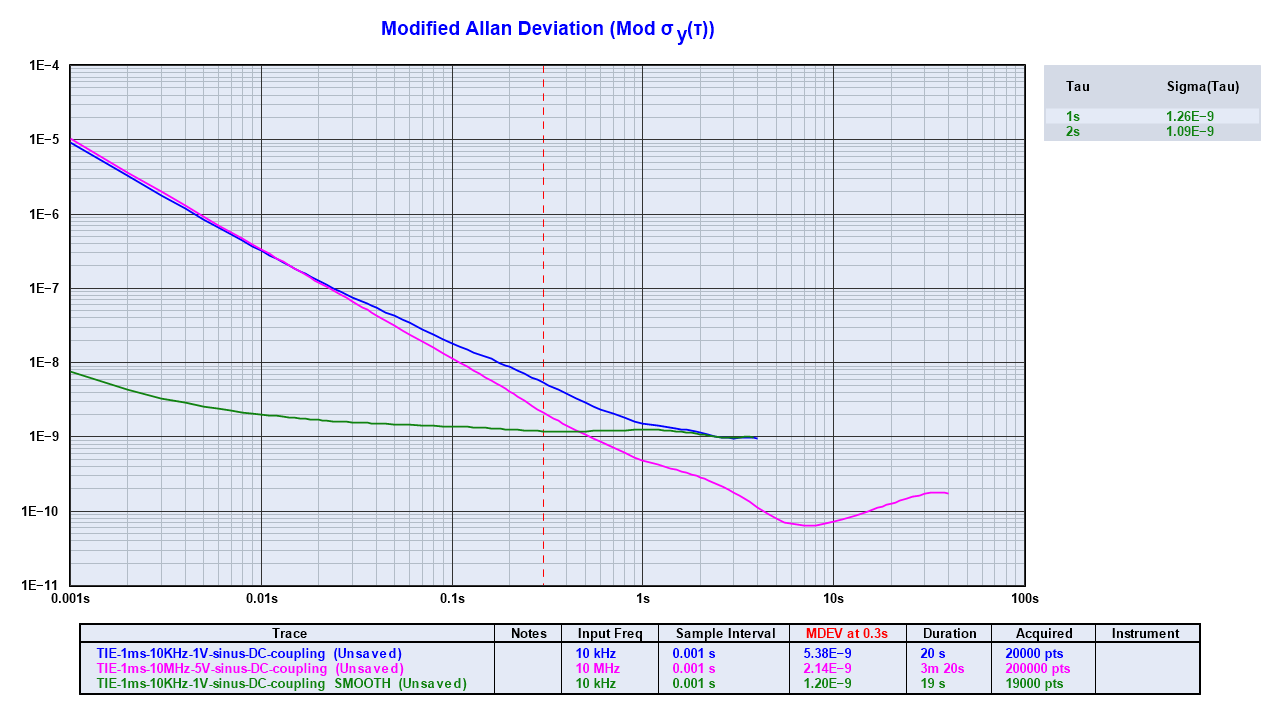
\includegraphics[width=1\textwidth]{mod_allan_last_part3.png}
    \label{fig:15Vsg_10x_mod_allan_dev}
      \caption{TIE measurements for 10 MHz/KHz 1 ms sample rate 1/5V Modified Allan Deviation}
\end{figure}

\end{document}                     